% !Mode:: "TeX:UTF-8"
% 本章介绍自动驾驶基础知识、高精地图作用与使用范围等等
\thispagestyle{empty}
\setcounter{page}{1}
\part{Basic Knowledge}
\thispagestyle{empty}
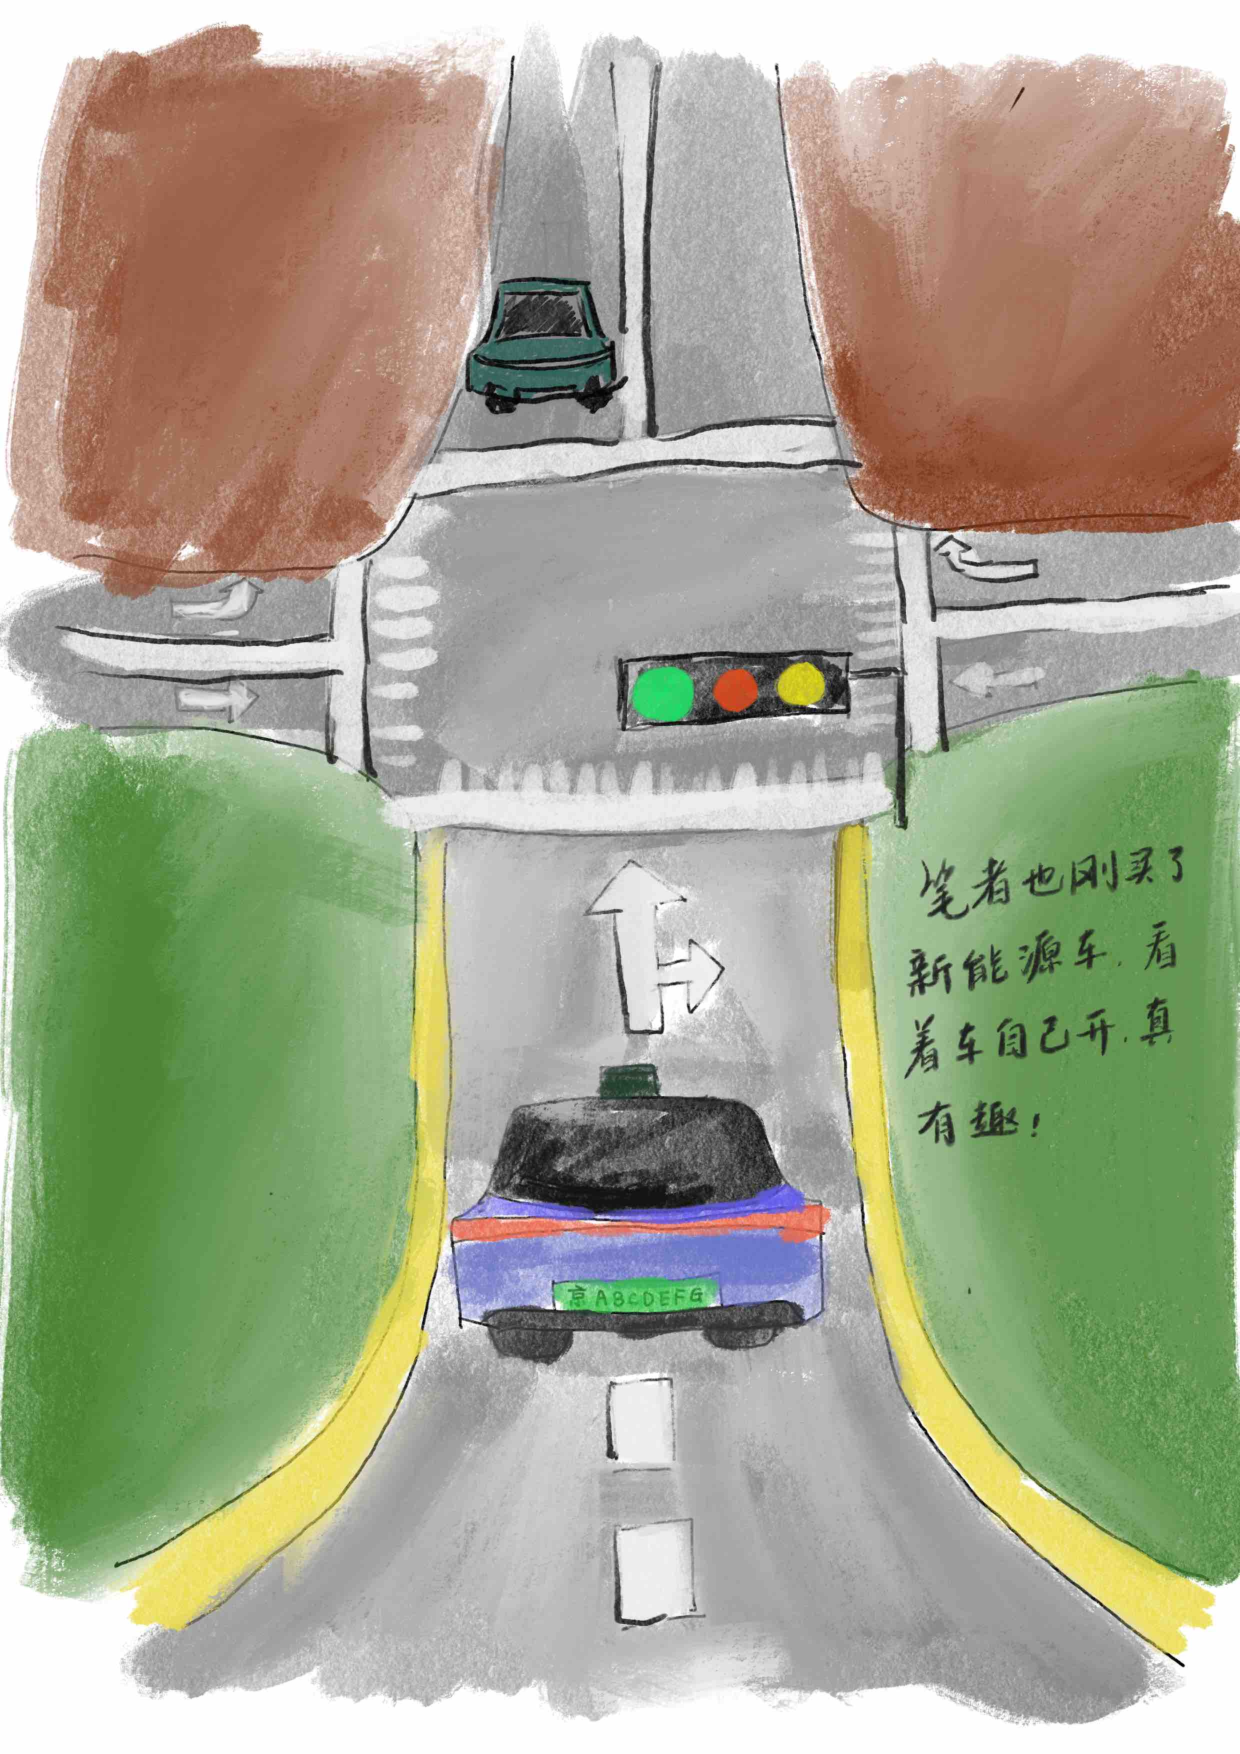
\includepdf[width=\textwidth]{art/ch1.pdf}

\newpage

\chapter{Autonomous Driving}
\thispagestyle{empty}
\setcounter{chapter}{1}
\section{Autonomous Driving Technologies}
\subsection{Autonomous Driving Capabilities and Grading}
Autonomous driving, as the name suggests, is the study of enabling vehicles to drive by itself. If you were to design an autonomous driving system, where would you start?

Although the internal structure of a car is highly complex, what humans actually need to operate is simply looking ahead, manipulating the steering wheel, accelerator, and brake pedals. If a computer program also learns to send signals to the steering wheel and pedals based on information from camera images, does it qualify as learning autonomous driving? If so, how should this program be designed?

In a naive conception, to enable a car to autonomously drive, one should first observe how humans perform driving behaviors. Humans primarily use vision to judge the relationships between their own vehicles and surrounding vehicles, pedestrians, and roads. They determine the direction of travel by observing lane markings and then use maps to determine long-term route planning. Similarly, autonomous vehicles should possess these abilities. Let's make a simple analogy:

\begin{enumerate}
	\item Autonomous vehicles should be able to identify the types of surrounding vehicles and pedestrians in real time, recognize road signs and signals, such as common lane markings, traffic lights, and traffic signs. This is called the \textbf{perception} capability of the vehicle \cite{Qian2020, Zhang2018}.
	\item The vehicle should be able to determine its own direction and position, as well as the positional relationship between itself and the aforementioned elements. This is also known as the \textbf{localization} capability of the vehicle \cite{Wei2020, Hungar2020, Wang2017}.
	\item The vehicle should be able to control the throttle, brake, steering wheel, and other actuators based on the aforementioned signal recognition results, and plan short-term and long-term driving routes. This is called the \textbf{planning and control} (P\&C) capability of the vehicle \cite{Sun2018, Viana2021}.
\end{enumerate}

However, despite addressing the same problems, the capabilities of humans and computers differ greatly. Throughout the long history of evolution, humans have developed extremely powerful spatial \textbf{perception} abilities. We can understand the vast majority of objects in our field of vision in an instant, with minimal errors. We also possess strong learning abilities; even when encountering unfamiliar objects, we instinctively avoid them. We can quickly understand the structure of the road ahead in any weather and scene, and even drive normally on roads without lane markings. We can also communicate with surrounding vehicles through lights and sounds, and predict their actions based on the behavior of other vehicles. In some defensive driving techniques, we can even infer potential dangers in blind spots. Due to these powerful understanding abilities, we can drive vehicles freely based solely on vision, without precise position and attitude information, unlike autonomous vehicles, which require expensive ranging devices like LiDAR, high-definition maps, and high-precision positioning to precisely control vehicle behavior (Figure \ref{fig:human-auto}).

\begin{figure}[!htp]
	\centering
	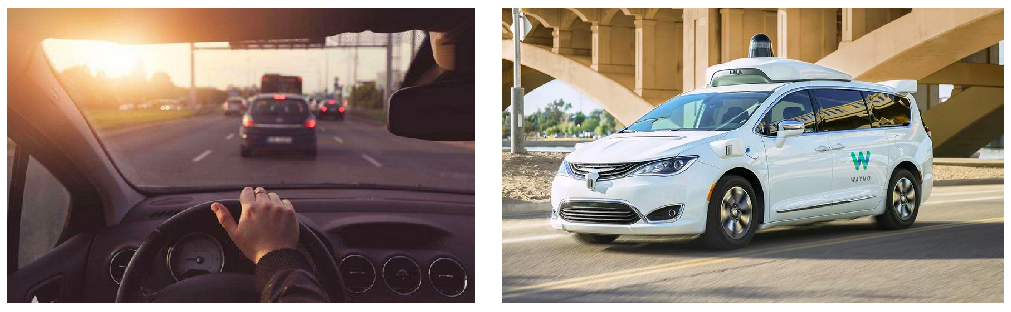
\includegraphics[width=\textwidth]{introduction/human-auto}
	\caption{Cars driven by humans versus cars driven autonomously. Humans can drive solely based on vision, while autonomous vehicles currently rely on high-precision ranging devices and backend high-precision map services.}
	\label{fig:human-auto}
\end{figure}

If we were to draw a comparison between birds and airplanes, our human driving abilities would resemble the effortless and natural flight of birds in the sky. However, for aircraft designers, should they make airplanes flap their wings like birds? The reality is quite different. Aircraft possess sophisticated control devices to manipulate airflow over their wings to generate the necessary lift; they also have precise measuring instruments to determine their own attitude and use modern control methods to maintain the desired orientation. The relationship between autonomous and human-driven vehicles is very similar to that of airplanes and birds. We can draw upon certain human abilities to design autonomous driving systems, but the resulting autonomous vehicles will inevitably differ significantly from human-driven ones. We don't necessarily need autonomous vehicles to behave exactly like human-driven ones. Autonomous vehicles should have their own design and operational logic.

In fact, autonomous driving vehicles are already capable of providing automated driving experiences. In several major cities in China (such as Beijing, Shanghai, Changsha, Chongqing, Wuhan, Shenzhen, among others), autonomous taxis (Robotaxis) has been opened to the public and can be experienced at any time. If you were to sit in an autonomous vehicle, you would notice that the steering wheel turns automatically, and braking and acceleration do not require human intervention. You might realize that if the vehicle were entirely controlled by a computer, there would be no need to install those steering wheels, pedals, or central control panels in the car. Additionally, you can see on the vehicle screen the planned route, surrounding vehicles and pedestrians, and data provided by HD maps. Since 2018, these vehicles have undergone several years of pilot testing but have not yet reached mainstream consumers.

On the other hand, if you were looking to buy a vehicle soon, most vehicles would advertise their autonomous driving features. They can automatically maintain a fixed speed on highways, eliminating the need for you to operate the accelerator; they can also automatically steer to keep the vehicle in the center of the lane, relieving you of steering duties. Some vehicles even offer features like lane change assistance or automatic lane changing, so you can leave lane changing to the vehicle. They can even handle automatic following in congested traffic conditions. These features indeed assist drivers in vehicle operation. Moreover, these vehicles are tangible and can be purchased at widely accepted prices. Most of them use purely visual or predominantly visual sensor solutions.

Are all of these considered ``autonomous driving''? If so, why is it difficult to purchase the former now, while the latter can appear directly on the consumer market?

This is precisely the situation that autonomous driving faces today: if we want to achieve driving capabilities similar to humans and have vehicles drive entirely on their own without the need for drivers, it requires a hefty price to implement such functionality. This cost could be attributed to laser radar sensors, backend map services, machine costs, research and development investments, and so on. When vehicles no longer require drivers, many business models will change accordingly. Taxi companies will no longer need drivers, food delivery companies will no longer need delivery personnel, and all operational personnel will only need to maintain autonomous driving vehicles. On the other hand, if we want to keep the price of vehicles within the reach of consumer-grade vehicles by using inexpensive, practical sensors, then we must acknowledge the current lack of reliability in existing algorithms, necessitating human driver supervision and intervention at any time, unable to completely replace human drivers. In fact, the entire autonomous driving industry is currently exploring along these two paths. The former path is highly likely to lead to fully autonomous driving, but currently, it seems too expensive to be directly targeted at consumers; the latter path is known as the ``incremental'' route, which is being used by various vehicle manufacturers, but it still has a significant distance from fully autonomous driving and is not suitable for tasks that require fully autonomous driving capabilities.

This divergence in paths reminds us that sometimes when discussing autonomous driving, different parties may not necessarily be talking about the same tasks. In fact, if we only care about ``some'' autonomous driving tasks, such as automatic following, lane keeping, and automatic lane changing, they do not require very complex technology or sensors. Although we sometimes refer to these vehicles as ``autonomous driving'' vehicles, and their manufacturers are also willing to claim that they are ``fully autonomous driving,'' they still belong to the category of ``assisted driving'' functions according to standards. This also reminds us that there should be a clear and standardized delineation of autonomous driving capabilities.

In the international arena, researchers have long classified vehicles into five levels of autonomy, from Level 1 to Level 5 (SAE classification\footnote{Classification by the Society of Automotive Engineers, see SAE Standard J3016-202104: \url{https://www.sae.org/standards/content/j3016_202104}.}), as shown in \autoref{table:SAE}. Similar to this, China has its own ``Classification of Automotive Driving Automation''\footnote{See: GB/T: 40429-2021.}, the summary of which is presented in \ref{table:GBT-Chinese}. Generally, the various standards for classifying autonomous driving capabilities are primarily based on the following two points:

\begin{enumerate}
\item Whether the system requires human intervention, also known as \textbf{intervention}. \textbf{Assisted driving systems} require the driver to take over when intervention is needed, while \textbf{autonomous driving systems} strive to operate without the need for human intervention, allowing the removal of driver equipments such as steering wheels and pedals. This is the key distinction between Level 2 and above Level 3 autonomous driving capabilities.
\item Whether the system operates in limited scenarios or can function in most normal scenarios relative to human drivers. This is the key difference between Level 4 and Level 5.
\end{enumerate}

\begin{table}[h]
	\footnotesize
	\caption{SAE Automated Driving Levels}
	\label{table:SAE}
	\centering
	\begin{threeparttable}
	\begin{tabular}{|c|ccc|ccc|}
		\hline Level & L0 & L1 & L2 & L3 & L4 & L5 \\\hline
		Responsiblity & \multicolumn{3}{c}{Driver} & \multicolumn{3}{c|}{Computer} \\\hline
		Intervention & \multicolumn{3}{c|}{at all times} & when required & \multicolumn{2}{|c|}{not required} \\\hline
		Typical Func. & \makecell[l]{AEB\\BSD\\ LDW \\ ALC} & \makecell[l]{LCC\\ACC} & LCC+ACC & \makecell[l]{Traffic Jam Driving\\Auto Parking\\Auto Summoning} & \makecell[c]{Robotaxi\\Robotruck} & all conditions \\\hline
	\end{tabular}
	\begin{tablenotes}
	\item Abbreviations: LDW: Lane Departure Warning, ACC: Adaptive Cruise Control, LCC: Lane Centering Control, BSD: Blind Spot Detection, AEB: Automatic Emergency Braking, ALC: Auto Lane Change.
	\end{tablenotes}
	\end{threeparttable}
\end{table}

\begin{table}[h]
	\footnotesize
	\caption{China Classification of Automotive Driving Automation}
	\label{table:GBT-Chinese}
	\centering
	\begin{tabular}{|c|c|c|}
		\hline Driving Level & Name & Main Contents \\\hline
		L0 & Emergency Assist. & \makecell[l]{Detection and response capabilities for certain events} \\
		L1 & Partial Driver Assist. & \makecell[l]{Continuous execution of lateral and longitudinal control} \\
		L2 & Combined Driver Assist. & \makecell[l]{Continuous execution of lateral and longitudinal control} \\
		L3 & Conditionally Auto. Driving & \makecell[l]{Continuous execution of all driving tasks} \\
		L4 & Highly Auto. Driving & User may refrain from taking over \\ 
		L5 & Fully Auto. Driving & Can autonomously drive in any environment \\\hline
	\end{tabular}
\end{table}

Therefore, although there are five to six levels in terms of classification, for professionals in the field of autonomous driving, the main concern lies in Levels 2 and 4. Level 2 autonomous driving vehicles can be directly targeted at consumers, enhancing driving comfort to a certain extent based on traditional vehicles. The functionalities currently achieved at Level 2 are not far from current laws and regulations and are gradually being popularized in some new car models. On the other hand, Level 4 vehicles should be capable of unmanned driving in most scenarios, able to address some business needs for automation, which is also considered by many researchers as a form of ``driverless'' mode. Although within the broad definition, both Level 2 and Level 4 are part of autonomous driving, in practical terms, there are fundamental differences in module design and implementation between them. Level 4 autonomous driving is most concerned with the \textbf{intervention rate}, requiring that the vehicle cannot be taken over by human without cause, thus placing high demands on various algorithm performances. On the other hand, all functions of Level 2 autonomous driving can be taken over by humans, thus emphasizing the recognition of which scenarios are \textbf{valid scenarios}, where Level 2 functionalities can be activated. Due to human intervention, Level 2 is much more tolerant of most algorithm metrics, placing greater emphasis on the presence of functions rather than complete automation.


\begin{figure}[!htp]
	\centering
	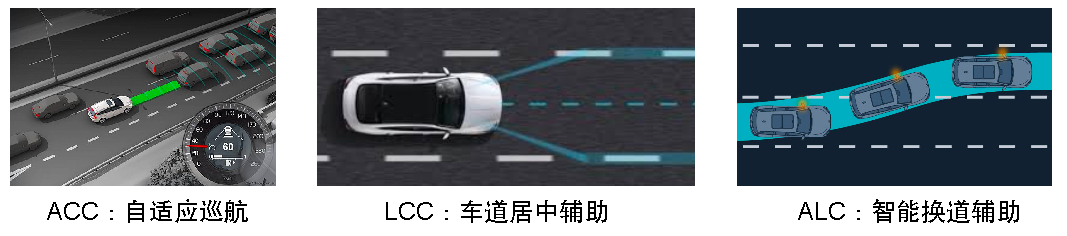
\includegraphics[width=1.0\textwidth]{introduction/l2-tasks}
	\caption{Typical L2 tasks: ACC, LCC, ALC. }
	\label{fig:l2-tasks}
\end{figure}

\subsection{Typical L4 Tasks}
L2 or L4, that is the question.

However, this question shouldn't be answered by technical personnel. We should first ask, does a certain type of vehicle really need to drive completely autonomously? In some scenarios, the answer is ``yes''. \textbf{Automation} is the core functionality of these vehicles. Without full automation, these vehicles lose their raison d'être. In other scenarios, we might say ``not necessarily.'' What we need more is safe driving with computers helping to \textbf{alleviate burdens}. If computers can provide more advanced functions, we are willing to accept them, but we also need to consider the cost of these functions. If the cost is too high, consumers won't buy it.

\begin{figure}[!t]
	\centering
	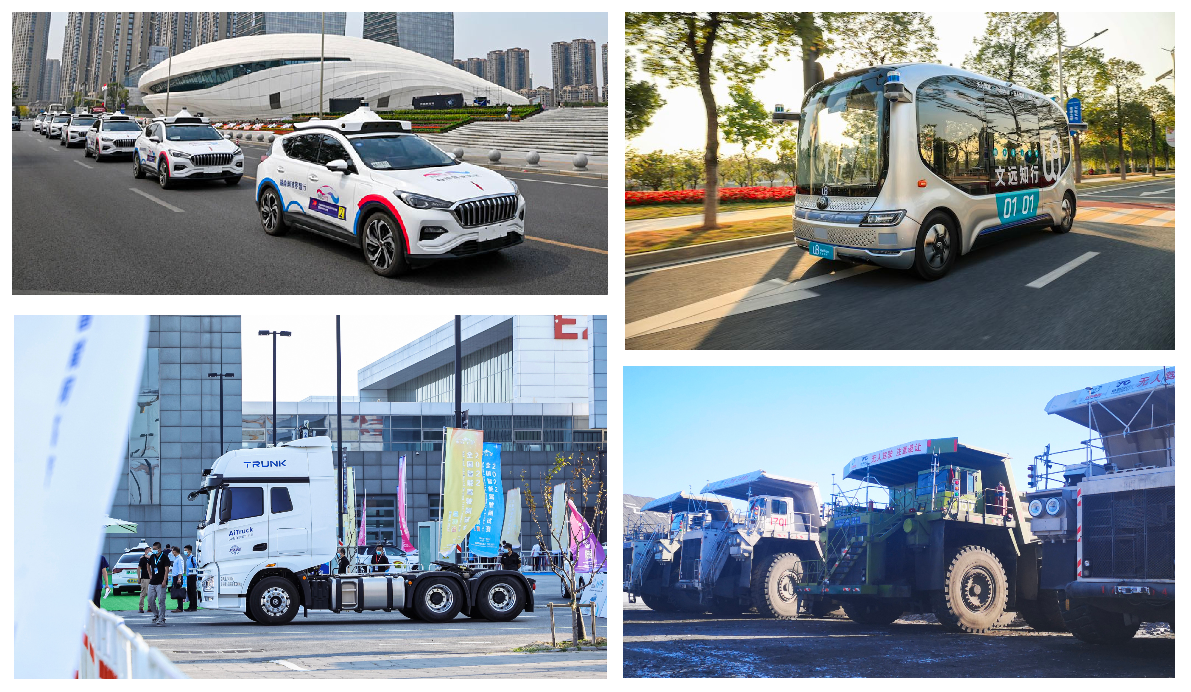
\includegraphics[width=1.0\textwidth]{introduction/l4-robotaxi}
	\caption{Some applications of L4 passenger vehicles: autonomous taxis, buses, trucks, mining trucks}
	\label{fig:l4-robotaxi}
\end{figure}

The former belongs to typical L4 applications, and the entity doesn't have to be limited to \textbf{vehicles}. In a broad sense, as long as a chassis carries sensors and has a certain level of automation, it can be considered a form of autonomous driving vehicle. From this perspective, whether the entity is a car or carries passengers is not the key to distinguishing autonomous driving. Whether the tasks they perform require \textbf{full automation} is the key to distinguishing their autonomous driving capabilities. For example, an autonomous delivery vehicle's primary function is to autonomously deliver items to users. If this function isn't fully automated and still requires a driver's cooperation, then the business loses its main feature. An autonomous cleaning vehicle's main function is to automatically cover cleaning in fixed scenes. If this process still requires human involvement, it's not meaningful. For these businesses, \textbf{removing the driver} is their most important feature, so they belong to core L4 applications. These vehicles are not designed with driver cabins or driver positions (Figure~\ref{fig:l4-lowspeed}).


\begin{figure}[!t]
	\centering
	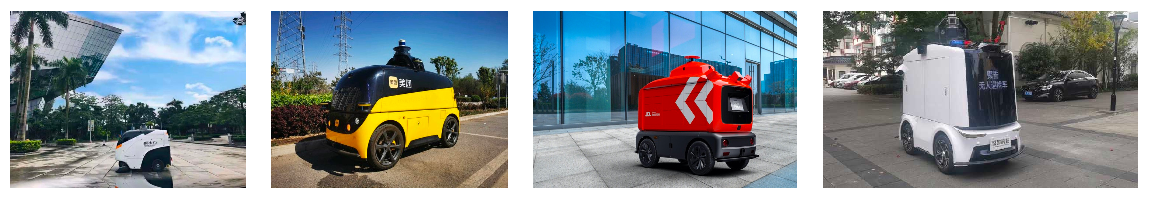
\includegraphics[width=1.0\textwidth]{introduction/l4-lowspeed}
	\caption{Low-speed L4 applications: sweepers, delivery bots, patrol robot}
	\label{fig:l4-lowspeed}
\end{figure}

On the other hand, we can also ask, do taxis need autonomous driving? Do trucks need autonomous driving? If there are no drivers, taxis can be operated solely by taxi companies, and trucks can also be operated solely by logistics companies, without the need to recruit drivers, only requiring vehicle maintenance. This business model is called Robotaxi and Robotruck, which is a completely different way from existing commercial models (see Figure~\ref{fig:l4-robotaxi}). It imposes strict requirements on autonomous driving. Once a vehicle experiences a failure and requires human intervention, in the absence of a driver on board, it's difficult to have a human driver intervene in a timely manner, and a takeover event could easily turn into an accident.

Applications such as Robotaxi, Robotruck, Robobus, etc., technically also belong to L4 autonomous driving. Compared to autonomous driving vehicles for cleaning, delivery, inspection, etc., they have higher requirements for autonomous driving safety, stricter requirements for overall vehicle system stability, lower tolerance for risks and failures, and require more perception, high-precision positioning, mapping, and other technical support. If a low-speed vehicle experiences a failure, it won't directly lead to casualties, and most of the time, it can be remotely managed by technical personnel. However, if a passenger-carrying vehicle experiences an accident, the consequences can easily have substantial impacts at the company or even the community level. So, we ask, can the current level of technology support applications like Robotaxi? Unfortunately, this question currently does not have a definitive answer.

On one hand, autonomous driving systems are complex systems, unlike traditional electronic or mechanical switches, where it's easy to provide a functional safety verification plan or give clear reasons for failures. If an autonomous driving vehicle fails to recognize a vehicle in front and collides, within the current theoretical framework, we can't explain \textbf{why the system failed to recognize the vehicle ahead}. It's just a phenomenon that occurs in reality. Perhaps if a certain value in a certain program is increased by 0.001, this phenomenon won't occur, but it may make it impossible to recognize vehicles of a different color in different weather conditions. There are hundreds of millions of parameters like this, none of them have names, and they are connected and calculated in a way arbitrarily stipulated by humans. It's difficult to attribute the occurrence of a specific result to a parameter being too large or too small, or the calculation sequence between them not being reasonable enough. A brake system is almost impossible to fail, but a perception system is almost impossible to be 100\% correct. In short, autonomous driving systems are difficult to precisely analyze what failure at a certain point may lead to what phenomenon, and provide convincing reasons, like traditional mechanical and electronic systems.

On the other hand, if it's difficult to verify the safety of autonomous driving vehicles from a theoretical level, can we statistically measure the stability of autonomous driving systems at an experimental level? This is indeed what many autonomous driving companies are doing now. Most L4 autonomous driving companies will statistically analyze the relationship between vehicle mileage and takeover times, for example, calculating the \textbf{miles per intervention} (MPI)\footnote{Sometimes also called miles per disengagement, MPD.}, to measure the stability of the system. In the 2021 report of the California Department of Motor Vehicles (DMV) on autonomous driving, the MPI of some Chinese companies has reached the level of thousands to tens of thousands of kilometers (see Table~\ref{table:l4-mpi})\footnote{Source: \url{http://www.evinchina.com/articleshow-217.html}}. We generally believe that MPI is indeed an indicator of the overall autonomous driving capability of a vehicle, but so far, there is no very open and fair MPI testing method, and what we can see more are self-testing reports from various companies. They lack unified testing environments and standardized criteria for when to intervene. In terms of quantity and mileage, compared to traditional mass-produced vehicles, most L4 autonomous driving companies only have fleets consisting of dozens or hundreds of vehicles, and their road test scenarios are usually relatively simple. Compared to traditional manufacturers with monthly sales of tens of thousands of vehicles, their accumulated test mileage and number of scenarios are very limited.

%\begin{figure}[!t]
%	\centering
%	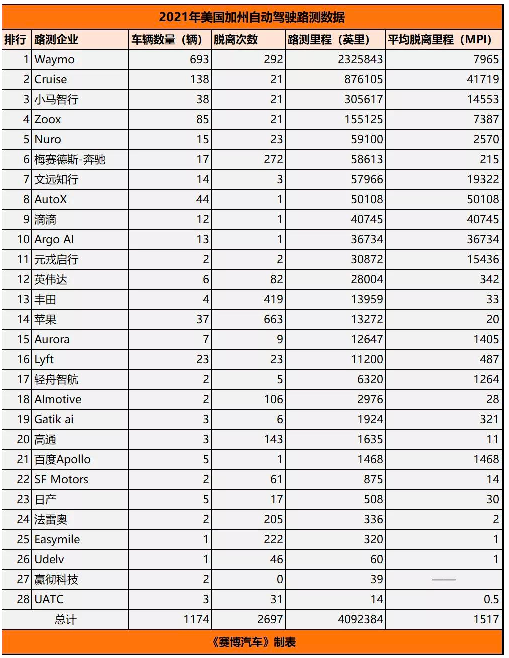
\includegraphics[width=0.7\textwidth]{introduction/l4-mpi}
%	\caption{2021 report of the California Department of Motor Vehicles (DMV) on autonomous driving}
%	\label{fig:l4-mpi}
%\end{figure}

\begin{table}[!t]
	\footnotesize
	\caption{2021 report of the California Department of Motor Vehicles (DMV) on autonomous driving}
	\label{table:l4-mpi}
	\centering
	\begin{tabular}{c|llll}
		\hline\hline Company & Num. of cars & Num. of Invent. & Miles & MPI \\\hline
		Waymo & 693 & 292 & 2325843 & 7965 \\\hline
		Cruise & 138 & 21 & 876105 & 41719 \\\hline 
		Pony.ai & 38 & 21 & 305617 & 14553 \\\hline
		Zoox & 85 & 21 & 155125 & 7387 \\\hline 
		Nuro & 15 & 23 & 59100 & 2570 \\\hline
		Mercedes-Benz & 17 & 272 & 58613 & 215 \\\hline 
		WeRide & 14 & 3 & 57966 & 19322 \\\hline 
		AutoX & 44 & 1 & 50108 & 50108 \\\hline
		DiDi & 12 & 1 & 40745 & 40745 \\\hline 
		Argo AI & 13 & 1 & 36734 & 36734 \\\hline 
		DeepRoute.ai & 2 & 2 & 30872 & 15436 \\\hline 
		Nvidia & 6 & 82 & 28004 & 342 \\\hline 
		Toyota & 4 & 419 & 13959 & 33 \\\hline
		Apple & 37 & 663 & 13272 & 20 \\\hline 
		Aurora & 7 & 9 & 12647 & 1405 \\\hline 
		Lyft & 23 & 23 & 11200 & 487 \\\hline 
		Almotive & 2 &106 & 2976 & 28 \\\hline 
		Gatik ai & 3 & 6 & 1924 & 321 \\\hline 
		Qualcomm & 3 & 143 & 1635 & 11 \\\hline 
		Apollo & 5 & 1 & 1468 & 1468 \\\hline 
		SF Motors & 2 & 61 & 875 & 14 \\\hline 
		Nissan & 5 & 17 & 508 & 39 \\\hline 
		Valeo & 2 & 205 & 336 & 2 \\\hline 
		Easymile & 1 & 222 & 320 & 1 \\\hline
		Udelv & 1 & 46 & 60 & 1 \\\hline
		Inceptio.ai & 2 & 0 & 39 & - \\\hline 
		UATC & 3 & 31 & 14 & 0.5 \\\hline\hline
	\end{tabular}
\end{table}

The dilemma of whether to have vehicles first or autonomous driving technology first is facing all L4 autonomous driving companies. Without a sufficient number of vehicles, it's difficult to prove that an autonomous driving system is stable enough, and thus challenging to truly implement businesses like Robotaxi; however, if we focus solely on the vehicle itself without paying attention to autonomous driving technology, it's also challenging to attract enough technical talents and cultivate the team's technical capabilities. Several years ago, it was a common problem that L4 technology companies didn't understand vehicles, and vehicle manufacturers didn't understand autonomous driving. Doing both requires enormous scale and determination, while collaboration between two different companies requires a high level of trust. Fortunately, major vehicle manufacturers have begun to pay attention to autonomous driving-related businesses (although currently focused on the easier-to-implement L2 business), and L2-related functionalities have been integrated into many vehicle models. Many practitioners also believe that as autonomous driving technology matures, L2 functionalities will gradually become richer and gradually approach L4 capabilities. Suppliers of autonomous driving-related sensors, algorithms, chips, and hardware will also play active roles in various vehicle models.

Even after overcoming technical issues, businesses like Robotaxi still face practical legal and social issues. After all, if L4 vehicles are widely deployed, other drivers will face the challenge of how to interact with driverless vehicles\footnote{Throughout this book, the term \textbf{driverless vehicles} generally refers to L4 autonomous driving vehicles.}. Will driverless vehicles understand the intentions of other vehicles changing lanes or overtaking? Will they avoid vehicles driving in the wrong direction? Will they detour around road sections undergoing sudden construction? Will they recognize children who have fallen on the road? Legally, how should the responsibility of driverless vehicles be defined if they collide with other vehicles? Should the responsibility lie with the developer of the driverless vehicle? Should the developers be held accountable if the collision occurs because the perception system failed to correctly identify pedestrians, or because the map annotation personnel incorrectly annotated the speed limit information of a road section, or because the satellite signal was weak that day, causing the vehicle to enter the wrong lane? These are questions that may be encountered in reality but are difficult to answer. In vehicles with human drivers, most safety responsibilities ultimately fall on the driver. Once the subject becomes a driverless vehicle, these responsibilities are difficult to distribute among various modules. It's unlikely that any company currently has the ability to assume these responsibilities on behalf of autonomous driving development companies. In short, discussions on many legal, ethical, and social issues related to autonomous driving will continue for many years to come.

However, autonomous driving still represents the direction of future technological advancement. Its overall prospects are promising, albeit with inevitable challenges along the way. Future passenger vehicles, low-speed vehicles, and robots will become increasingly intelligent, taking on more and more tasks in daily life. A series of technical issues derived from autonomous driving will also be fully addressed and discussed by researchers in various fields. Many things that appeared in science fiction movies will gradually become familiar landscapes in the coming years. For example, restaurant robots that the author fantasized about during their studies were once among the representatives of science fiction, but now they are widely present in major shopping malls, and major suppliers have begun price wars. Will autonomous driving vehicles also experience this situation in the coming years? We wait and see.

\section{Localization and Mapping in Autonomous Driving}
\subsection{Why L4 Needs Localization and Mapping}
This book primarily discusses the localization and mapping technologies in L4 autonomous driving. Before delving into the details, readers might ask a fundamental question: why does autonomous driving require localization and mapping?

That's an excellent question. My answer is, if high-precision localization and mapping weren't necessary for autonomous driving, that would be ideal. Unfortunately, at the current technological level, achieving low intervention rates in L4 autonomous driving still requires the use of high-precision localization and mapping. Conversely, if we're discussing L2 autonomous driving, which doesn't prioritize intervention rates, high-precision localization and mapping may not be necessary (although some L2 systems are also using high-precision maps) \cite{Zhang2021, Ort2020, Can2020}. This contradicts the current level of intelligence and reliability. The smarter it is, the less reliable it becomes; the more reliable it is, typically meaning simpler in structure, the less intelligent it is. If we choose to accept the results of AI, we must also accept the mistakes made by AI. As for when L4 is needed and when L2 is needed, we've discussed this earlier.

\begin{figure}[!t]
	\centering
	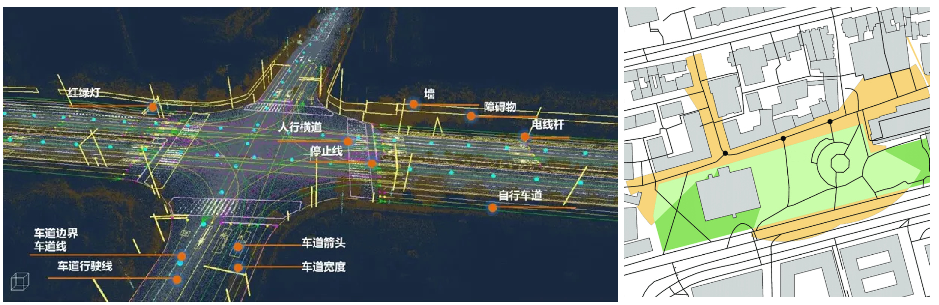
\includegraphics[width=1.0\textwidth]{introduction/hdmap}
	\caption{Differences between high-definition maps and traditional electronic navigation maps. Navigation maps represent roads and intersections using polygons and vectors, while high-definition maps also accurately mark lane positions, stop line positions, and provide detailed information about surrounding objects.}
	\label{fig:hdmap}
\end{figure}

Why does L4 need high-definition maps? This is because L4 and L2 have different goals. L2 autonomous driving doesn't concern itself with intervention rates, whereas achieving low intervention rates is the primary goal of L4, which determines that their technological paths have fundamental differences. L4-related technologies exhibit strong determinism. Many behaviors that may seem acceptable at the L2 level, such as turning into the wrong lane at an intersection or misreading a traffic light, would result in intervention in L4 and are not allowed to occur. Consequently, L2 leans more toward real-time perception and may even use perception results directly to construct a bird's eye view (BEV) \cite{Sun2020, Ng2020, Hendy2020}, while L4 relies on offline maps \cite{Levinson2010, Wolcott2014, Matthaei2014}. In simple terms, L2 is more like ``driving while looking at the road,'' whereas L4 is ``driving in the map in the mind.'' ``Driving while looking at the road'' has the advantage of very direct logical relationships, closer to human behavior, but the disadvantage is dealing with the limitations and uncertainties of computer detection results. Vehicle cameras typically only see the ground lane lines a few dozen meters ahead. They may also be obscured by other vehicles, submerged in puddles, or, due to lighting conditions, shadows of roadside guardrails may be mistaken for lane lines. These outcomes could affect the vehicle's autonomous driving behavior, and these uncertainties must be considered at the control and decision-making levels. In contrast, high-definition maps in L4 are meticulously annotated by humans, with accurate positions for each lane. It's predetermined which lane they will continue onto, which direction to turn at intersections, and which traffic light to look at in three-dimensional space \cite{Ghallabi2018}. Even if no lane lines are visible in real-time images, L4 vehicles can accurately follow straight lines in the map \cite{Yang2018}. This approach comes with two costs: first, we need to create such a high-definition map in advance; second, we need to know our accurate position in this map \cite{Spangenberg2016, Levinson2007}.

High-precision localization and mapping represent a strict, accurate concept. On the flip side, it brings about rigid, cumbersome business burdens. Maps essentially transform those limited, uncertain perception elements into static, precise data information through manual or post-processing methods (Figure \ref{fig:hdmap}). Maps carry out similar tasks to real-time perception but can provide correct results across unlimited ranges, greatly reducing the burden of perception \cite{Seif2016}. Therefore, some have said that maps are a cheating sensor, essentially providing the answers directly to autonomous driving vehicles. With high-definition maps, the vehicle's burden of perception can be significantly alleviated. We only need to focus on dynamic pedestrian and vehicle information, without worrying about the shape and topology of road lanes. However, the balance between maps and perception is constantly changing. Some companies' high-definition maps are richer than others, even including information about obstacles, flowerbed shapes, etc., while others' solutions require the perception module to detect this information. Perhaps in the near future, the balance between maps and perception will change with technological iterations.

In current L4 autonomous driving solutions, most task elements are tied to maps. When users want to drive from point A to point B in a city, the autonomous driving vehicle first generates a lane-level path from point A to point B on the map. This path is different from the common navigation systems we're familiar with; it's at the lane level. The navigation system calculates which road, which intersection, and which lane to turn into. When executing autonomous driving tasks, the vehicle also strives to ensure that the actual executed path aligns with the results of high-definition map navigation. For this reason, the vehicle needs to know its real-time position on the map, which requires high-precision localization within lanes.

\subsection{Contents and Production of High-Definition Maps}

High-definition maps are essentially \textbf{structured data} \cite{Zhou2021}. Their basic elements consist of sections of lanes in the real world, as depicted in Figure \ref{fig:hdmap-lane}. Various questions about lanes can be asked, such as:
\begin{enumerate}
	\item What is the geometric shape of this lane? Is it straight, with bends, or curved?
	\item Which lane is to its left, and which is to its right?
	\item What is the speed limit? Is it a straight lane or a turning lane?
	\item Is it a motorized lane or a non-motorized lane?
	\item Which lanes is it connected to? Are they sequentially connected, or are there forks or mergers?
\end{enumerate}

\begin{figure}[!t]
	\centering
	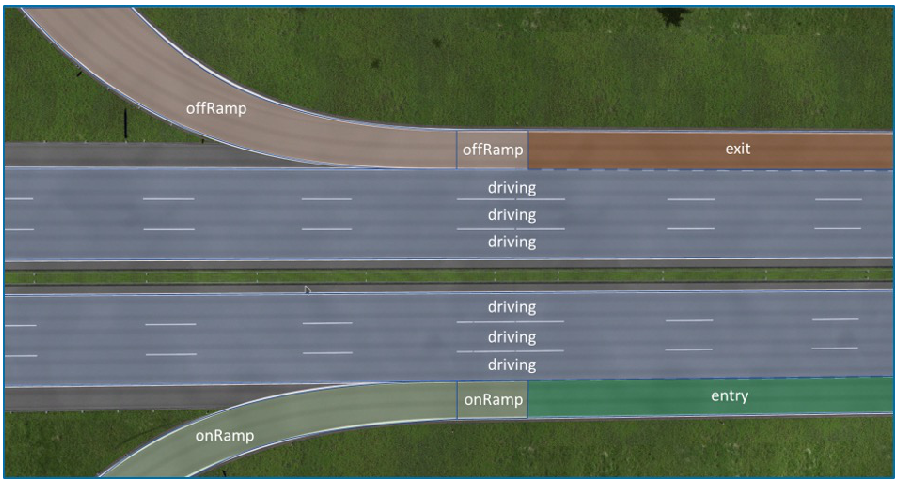
\includegraphics[width=0.7\textwidth]{introduction/hdmap-lane}
	\caption{Common lane information in high-definition maps}
	\label{fig:hdmap-lane}
\end{figure}

\begin{figure}[!t]
	\centering
	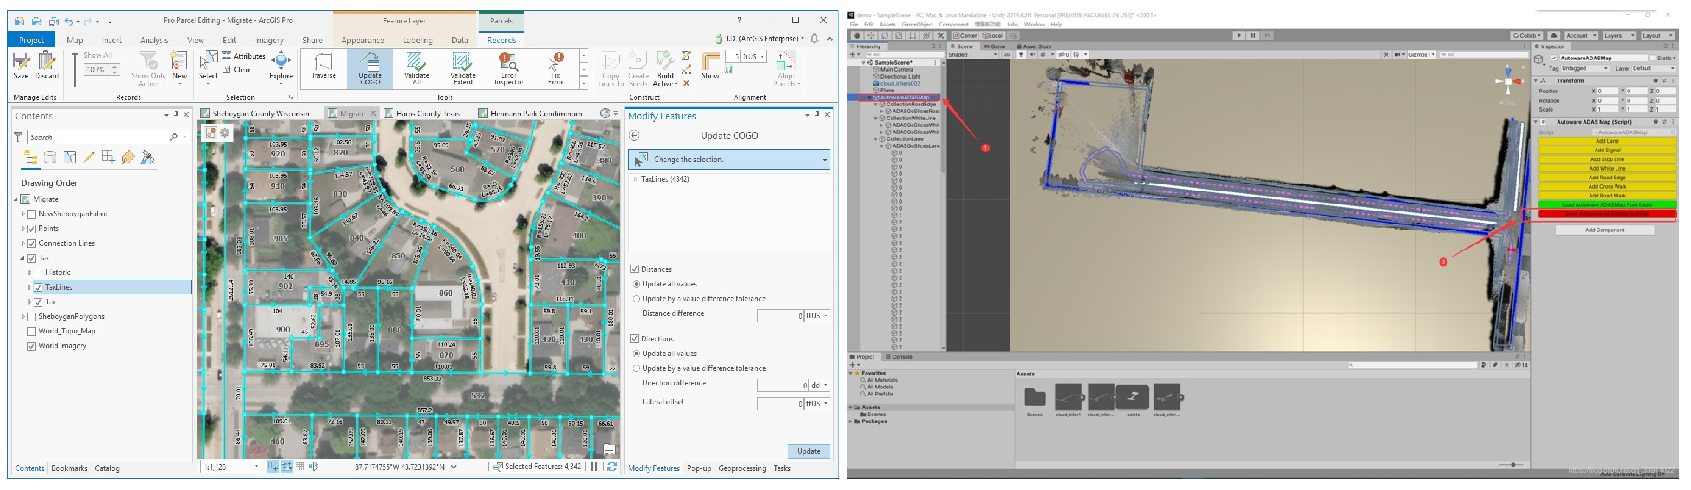
\includegraphics[width=1.0\textwidth]{introduction/hdmap-editor}
	\caption{Common high-definition map editing software: ArcGIS and Autoware Map Tool}
	\label{fig:hdmap-editor}
\end{figure}

Questions of this sort are easily described and stored using \textbf{structures} in programs. Various programming and markup languages support struct syntax, making high-definition map software compatible with multiple languages, including JSON, Protocol Buffers (protobuf), XML, and others. Describing a complete lane's information can be quite extensive and challenging. Researchers worldwide have therefore developed standards for high-definition maps. Common standards include OpenDrive \cite{Dupuis2010}, LaneLet2 \cite{Poggenhans2018}, and Apollo OpenDrive. These standards define ways to describe a lane, an intersection, and specifics of various traffic lights. Readers can refer to these standards for a comprehensive understanding of field information.

Most geometric elements in high-definition maps are described by points. For instance, a lane can be described by its center reference line plus its width, or by lines marking its left and right boundaries, which are composed of a series of lower-level points. The coordinates of each point can be expressed in terms of latitude and longitude or other global coordinate systems discussed later. Typically, they are represented by floating-point numbers. On the other hand, area-like elements can be described by polygons formed by multiple points, such as parking lots or buildings. Once this information is exported to files, it can be used for map rendering or for vehicle navigation and control.

Since high-definition maps are essentially made up of these lines and information, can't we generate them freely? Certainly, we can. We can even draw a road on paper and say its speed limit is 60 kilometers per hour; this can be considered a high-definition map, albeit with limited practical use. High-definition maps on computers are usually generated using specialized drawing software (such as ArcGIS, Autoware Map Tool, as seen in Figure \ref{fig:hdmap-editor}), and some companies may develop their own drawing software. You can certainly start from a blank area and draw a virtual map. However, if we want the map to correspond to the real world, we need to find a way to first obtain the three-dimensional structure or two-dimensional aerial view of the real world. These serve as the data source for real-world high-definition maps.

\begin{figure}[!t]
	\centering
	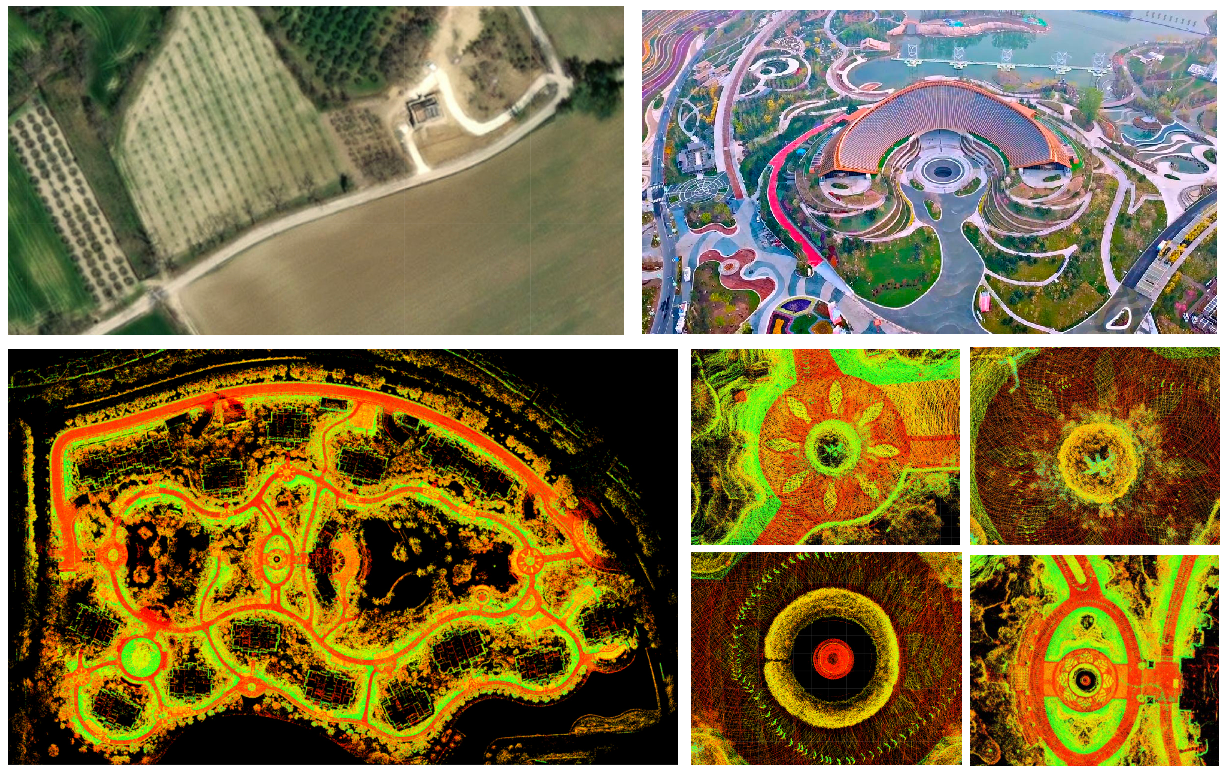
\includegraphics[width=1.0\textwidth]{introduction/hdmap-source-image}
	\caption{Data sources for high-definition maps: satellite imagery, drone aerial imagery, laser-generated point cloud maps (global and local)}
	\label{fig:hdmap-source}
\end{figure}

The two-dimensional or three-dimensional data from the real world mainly come from the following sources:

\begin{enumerate}
	\item Satellite imagery from remote sensing satellites. Satellite imagery can be obtained in various mapping software, but the highest resolution of civilian satellite imagery is at the level of a few meters, and images become blurred at around 10 meters. While they cover the entire globe and can be used for annotating electronic navigation maps, they are insufficient for high-definition maps, making it difficult to discern the specific positions of lanes and road surface details (see Figure \ref{fig:hdmap-source}, top left).
	\item Aerial imagery from drones. Drones equipped with high-precision positioning devices can take top-down photographs at any altitude, which are then stitched together to create aerial imagery. This imagery can be highly detailed, but its coverage is limited, and flying drones is prohibited in many areas.
	\item Three-dimensional map reconstruction using sensors carried by autonomous vehicles. The most common method is to use onboard LiDAR sensors to construct three-dimensional point clouds of the scene. These point clouds reflect the three-dimensional structure and brightness information of the scene and can effectively serve as a reference for map drawing. Since autonomous vehicles have relatively unrestricted ranges of travel, most autonomous driving companies use this method to construct point cloud maps \cite{Ghallabi2019, Ma2019}.
\end{enumerate}

Figure \ref{fig:hdmap-source} shows several different data sources. They follow a simple logic: the closer they are, the clearer they appear. Compared to remote sensing satellites orbiting tens of thousands of kilometers above the Earth, drones can hover tens of meters above the ground, while cars can directly capture images or measure distances in front of objects. Satellite images often struggle to discern road surface details, while drone images and LiDAR point clouds can reflect the texture of the road, the shapes of tree trunks and trees, and various small objects in the scene. Based on vehicle point clouds, we can annotate various detailed objects. If time permits, we can even annotate details such as the texture of tiles and the positions of tree trunks in high-definition maps.

\section{Introduction to SLAM in this Book}

The next question is how to use sensors onboard vehicles for high-precision point cloud reconstruction? What principles underlie this type of three-dimensional reconstruction? Apart from annotating maps, what other purposes do they serve? We will explore all of these questions throughout the content of this book. We will see that high-precision point clouds are the result of the combined action of a series of sensors. Their prices range from hundreds to hundreds of thousands, each serving different purposes. The core of the three-dimensional reconstruction system lies in estimating the vehicle's position and attitude at each moment, involving the vehicle's own \textbf{kinematic theory} and the \textbf{state estimation theory} used to estimate the vehicle's state using sensors. The following chapters of this book will introduce various sensor principles and methods in a certain order. The rough sequence is as follows:

\begin{enumerate}
	\item Firstly, we need to introduce some basic geometric knowledge, including the sensor coordinate systems on the vehicle and the coordinate systems of the Earth. At the same time, we will review the basic knowledge of state estimation theory, including the Kalman filter and nonlinear optimization theory. This part of the knowledge has been introduced in my previous book \cite{Gao2017}, so we will not elaborate further but only review. In particular, this book will mainly use properties on $\mathrm{SO}(3)$ when dealing with rotation variables. Readers need to maintain a certain proficiency in this part of the content. This is the content of Chapter 2 of this book.
	\item Chapters 3 and 4 will introduce two mainstream methods for processing \textbf{inertial measurement unit} (IMU) data. Chapter 3 introduces the classical Error State Kalman Filter (ESKF) and handles rotations in $\mathrm{SO}(3)$, while Chapter 4 mainly introduces preintegration methods. Since IMUs do not directly measure the physical state of the vehicle (translation and rotation) but rather measure their derivatives along the time axis (angular velocity and acceleration), we must introduce the differential relationship of the vehicle state and their various properties after integration. These are the main contents of Chapters 3 and 4.
	\item Chapters 5 to 7 introduce the content of laser SLAM. Chapter 5 mainly covers basic point cloud processing methods, including how to represent laser point clouds, how to find their nearest neighbors, and how to rasterize them. We will implement some classical data structures ourselves. Chapters 6 and 7 respectively introduce 2D and 3D laser SLAM methods. We will first implement some laser registration methods: 2D and 3D ICP, NDT, probability grid, etc., then manage them using sub-map methods, and finally add loop detection to form a complete SLAM system. Chapter 7 also introduces loosely coupled laser-inertial odometry.
	\item Chapters 8 to 10 introduce typical SLAM applications. Chapter 8 implements a tightly coupled laser-inertial odometry, each using an iterative error Kalman filter and a preintegration optimizer. Chapter 9 introduces offline point cloud map construction methods. We will rewrite some key algorithms into easily parallelized offline programs. Chapter 10 introduces methods for high-precision localization in existing point cloud maps. We will divide the point cloud map into small blocks in space and then use filters to achieve fusion localization of point clouds and inertial data.
\end{enumerate}

The above is the main content of this book. We mainly focus on the application of SLAM in autonomous driving around the aspects of inertial navigation and laser point clouds. Most vehicles on open roads or park roads can be mapped and located in this way. However, this book will not delve into the annotation part of maps in detail because they are mainly drawn manually and do not involve much algorithmic content\footnote{The automatic generation of high-definition maps is also a key research direction in the field of autonomous driving, but the methods are quite different from the content covered in this book, and the results are not yet mature. We will not delve into this topic. Readers can refer to related literature, such as \cite{Elhousni2020, Liao2022}.}.

Except for this chapter, the end of each chapter will include a certain number of exercises. Readers should allocate time for exercises according to their own learning progress.